\documentclass[11pt, mathserif]{beamer}

\geometry{paperwidth=13cm,paperheight=13cm}

\usepackage[
  nosetup,
  nothm
]{evan}
\usepackage{mathtools}
\usepackage{tikz}

\usetheme{Boadilla}
\usecolortheme{beaver}

\newtheorem{proposition}{Proposition}
\theoremstyle{definition}
\newtheorem{exercise}{Exercise}
\theoremstyle{remark}
\newtheorem{claim}{Claim}
\newtheorem{remark}{Remark}

% \usepackage{von}
% \renewcommand{\vonenvname}{example}

\title{Olympaid Graph Theory}
\subtitle{Irish Mathematical Olympiad Training}
\author{Adam Kelly (\texttt{ak2316@cam.ac.uk})}
\date{\today}

\usepackage{xcolor}
\definecolor{Smoke}{rgb}{0.96, 0.96, 0.96}
\setbeamercolor{background canvas}{bg=Smoke}

\begin{document}
\maketitle

\begin{frame}
  \section{Introduction}
\end{frame}

\begin{frame}
  \frametitle{Basic Definitions}

  \begin{definition}[Graph]
    A \vocab{graph} $G = (V, E)$ is a set $V$ of \vocab{vertices} and a set $E$ of unordered pairs of distinct vertices known as \vocab{edges}.
  \end{definition}

  \vspace{1cm}

  We have a natural way of drawing a graph:
  \begin{itemize}
    \item For each vertex we have a point in the plane,
    \item For each edge we draw a line between the corresponding pair of vertices.
  \end{itemize}
  
  
  \begin{example}[Path]
    The ordered pair $(V, E)$ where $V = \{1, 2, \dots, 6\}$ and $E = \{ (1, 2), (2, 3), \dots, (5, 6)\}$ is a graph.
  \begin{center}
      
  
        \tikzset{every picture/.style={line width=0.75pt}} %set default line width to 0.75pt        
  
        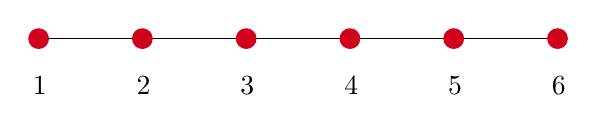
\begin{tikzpicture}[x=0.75pt,y=0.75pt,yscale=-1,xscale=1]
        %uncomment if require: \path (0,300); %set diagram left start at 0, and has height of 300
  
        %Straight Lines [id:da46250274214576614] 
        \draw    (175,115) -- (425,115) ;
        %Shape: Circle [id:dp08916666481415725] 
        \draw  [draw opacity=0][fill={rgb, 255:red, 208; green, 2; blue, 27 }  ,fill opacity=1 ] (220,115) .. controls (220,112.24) and (222.24,110) .. (225,110) .. controls (227.76,110) and (230,112.24) .. (230,115) .. controls (230,117.76) and (227.76,120) .. (225,120) .. controls (222.24,120) and (220,117.76) .. (220,115) -- cycle ;
        %Shape: Circle [id:dp7997596700799949] 
        \draw  [draw opacity=0][fill={rgb, 255:red, 208; green, 2; blue, 27 }  ,fill opacity=1 ] (270,115) .. controls (270,112.24) and (272.24,110) .. (275,110) .. controls (277.76,110) and (280,112.24) .. (280,115) .. controls (280,117.76) and (277.76,120) .. (275,120) .. controls (272.24,120) and (270,117.76) .. (270,115) -- cycle ;
        %Shape: Circle [id:dp04807433570988917] 
        \draw  [draw opacity=0][fill={rgb, 255:red, 208; green, 2; blue, 27 }  ,fill opacity=1 ] (320,115) .. controls (320,112.24) and (322.24,110) .. (325,110) .. controls (327.76,110) and (330,112.24) .. (330,115) .. controls (330,117.76) and (327.76,120) .. (325,120) .. controls (322.24,120) and (320,117.76) .. (320,115) -- cycle ;
        %Shape: Circle [id:dp6964194673091352] 
        \draw  [draw opacity=0][fill={rgb, 255:red, 208; green, 2; blue, 27 }  ,fill opacity=1 ] (370,115) .. controls (370,112.24) and (372.24,110) .. (375,110) .. controls (377.76,110) and (380,112.24) .. (380,115) .. controls (380,117.76) and (377.76,120) .. (375,120) .. controls (372.24,120) and (370,117.76) .. (370,115) -- cycle ;
        %Shape: Circle [id:dp5929377887646771] 
        \draw  [draw opacity=0][fill={rgb, 255:red, 208; green, 2; blue, 27 }  ,fill opacity=1 ] (420,115) .. controls (420,112.24) and (422.24,110) .. (425,110) .. controls (427.76,110) and (430,112.24) .. (430,115) .. controls (430,117.76) and (427.76,120) .. (425,120) .. controls (422.24,120) and (420,117.76) .. (420,115) -- cycle ;
        %Shape: Circle [id:dp5663003446831361] 
        \draw  [draw opacity=0][fill={rgb, 255:red, 208; green, 2; blue, 27 }  ,fill opacity=1 ] (170,115) .. controls (170,112.24) and (172.24,110) .. (175,110) .. controls (177.76,110) and (180,112.24) .. (180,115) .. controls (180,117.76) and (177.76,120) .. (175,120) .. controls (172.24,120) and (170,117.76) .. (170,115) -- cycle ;
  
        % Text Node
        \draw (171,132) node [anchor=north west][inner sep=0.75pt]    {$1$};
        % Text Node
        \draw (221,132) node [anchor=north west][inner sep=0.75pt]    {$2$};
        % Text Node
        \draw (271,132) node [anchor=north west][inner sep=0.75pt]    {$3$};
        % Text Node
        \draw (321,132) node [anchor=north west][inner sep=0.75pt]    {$4$};
        % Text Node
        \draw (371,132) node [anchor=north west][inner sep=0.75pt]    {$5$};
        % Text Node
        \draw (421,132) node [anchor=north west][inner sep=0.75pt]    {$6$};
  
  
        \end{tikzpicture}
  
    \end{center}
    This graph is known as $P_6$, a path on 6 vertices.
  \end{example}

\end{frame}

\section{Common Graphs}

\begin{frame}
  \frametitle{Common Graphs}

  There are some graphs that will appear repeatedly when doing graph theory problems, and we will define them now.
  

  \vspace*{1.25cm}

  \begin{definition}[Path]
    We define $P_n$ to be the graph 
    $V = \{1, \dots, n\}$, and $E = \{(1, 2), (2, 3), \dots, (n - 1, n)\}$ as shown.
    \begin{center}
      
  
        \tikzset{every picture/.style={line width=0.75pt}} %set default line width to 0.75pt        
  
        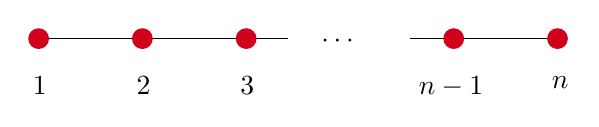
\begin{tikzpicture}[x=0.75pt,y=0.75pt,yscale=-1,xscale=1]
        %uncomment if require: \path (0,93); %set diagram left start at 0, and has height of 93
  
        %Straight Lines [id:da2966566565444405] 
        \draw    (354,35) -- (425,35) ;
        %Straight Lines [id:da13691249913110026] 
        \draw    (175,35) -- (295,35) ;
        %Shape: Circle [id:dp4038670448284668] 
        \draw  [draw opacity=0][fill={rgb, 255:red, 208; green, 2; blue, 27 }  ,fill opacity=1 ] (220,35) .. controls (220,32.24) and (222.24,30) .. (225,30) .. controls (227.76,30) and (230,32.24) .. (230,35) .. controls (230,37.76) and (227.76,40) .. (225,40) .. controls (222.24,40) and (220,37.76) .. (220,35) -- cycle ;
        %Shape: Circle [id:dp49083678213609794] 
        \draw  [draw opacity=0][fill={rgb, 255:red, 208; green, 2; blue, 27 }  ,fill opacity=1 ] (270,35) .. controls (270,32.24) and (272.24,30) .. (275,30) .. controls (277.76,30) and (280,32.24) .. (280,35) .. controls (280,37.76) and (277.76,40) .. (275,40) .. controls (272.24,40) and (270,37.76) .. (270,35) -- cycle ;
        %Shape: Circle [id:dp06755844317130888] 
        \draw  [draw opacity=0][fill={rgb, 255:red, 208; green, 2; blue, 27 }  ,fill opacity=1 ] (370,35) .. controls (370,32.24) and (372.24,30) .. (375,30) .. controls (377.76,30) and (380,32.24) .. (380,35) .. controls (380,37.76) and (377.76,40) .. (375,40) .. controls (372.24,40) and (370,37.76) .. (370,35) -- cycle ;
        %Shape: Circle [id:dp31955744853716384] 
        \draw  [draw opacity=0][fill={rgb, 255:red, 208; green, 2; blue, 27 }  ,fill opacity=1 ] (420,35) .. controls (420,32.24) and (422.24,30) .. (425,30) .. controls (427.76,30) and (430,32.24) .. (430,35) .. controls (430,37.76) and (427.76,40) .. (425,40) .. controls (422.24,40) and (420,37.76) .. (420,35) -- cycle ;
        %Shape: Circle [id:dp922206172324968] 
        \draw  [draw opacity=0][fill={rgb, 255:red, 208; green, 2; blue, 27 }  ,fill opacity=1 ] (170,35) .. controls (170,32.24) and (172.24,30) .. (175,30) .. controls (177.76,30) and (180,32.24) .. (180,35) .. controls (180,37.76) and (177.76,40) .. (175,40) .. controls (172.24,40) and (170,37.76) .. (170,35) -- cycle ;
  
        % Text Node
        \draw (171,52) node [anchor=north west][inner sep=0.75pt]    {$1$};
        % Text Node
        \draw (221,52) node [anchor=north west][inner sep=0.75pt]    {$2$};
        % Text Node
        \draw (271,52) node [anchor=north west][inner sep=0.75pt]    {$3$};
        % Text Node
        \draw (357,52) node [anchor=north west][inner sep=0.75pt]    {$n-1$};
        % Text Node
        \draw (421,52) node [anchor=north west][inner sep=0.75pt]    {$n$\ };
        % Text Node
        \draw (310,32) node [anchor=north west][inner sep=0.75pt]    {$\cdots $};
  
  
        \end{tikzpicture}
  
  
    \end{center}
    We call this a \vocab{path} on $n$ vertices, and say it has \vocab{length} $n - 1$.
  \end{definition}
  
\end{frame}

\begin{frame}
  \frametitle{Common Graphs}

  \begin{definition}[Cycle]
    We define $C_n$ (for $n \geq 3$) to be the graph  $V = \{1, \dots, n\}$, and $E = \{ (1, 2), \dots, (n - 1, n), (n, 1)\}$ as shown.
    \begin{center}
      
      
  
  \tikzset{every picture/.style={line width=0.75pt}} %set default line width to 0.75pt        
  
  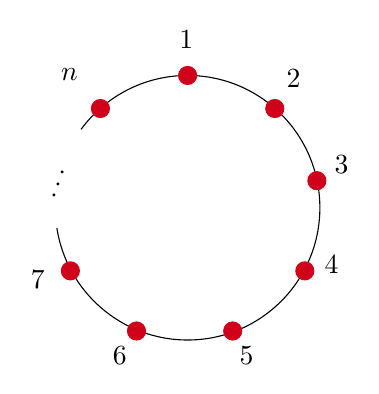
\begin{tikzpicture}[x=0.75pt,y=0.75pt,yscale=-1,xscale=1]
  %uncomment if require: \path (0,461); %set diagram left start at 0, and has height of 461
  
  %Shape: Arc [id:dp2939097210495426] 
  \draw  [draw opacity=0] (217.92,102.71) .. controls (229.52,86.97) and (248.19,76.75) .. (269.25,76.75) .. controls (304.45,76.75) and (332.98,105.28) .. (332.98,140.48) .. controls (332.98,175.68) and (304.45,204.21) .. (269.25,204.21) .. controls (237.36,204.21) and (210.94,180.77) .. (206.26,150.19) -- (269.25,140.48) -- cycle ; \draw   (217.92,102.71) .. controls (229.52,86.97) and (248.19,76.75) .. (269.25,76.75) .. controls (304.45,76.75) and (332.98,105.28) .. (332.98,140.48) .. controls (332.98,175.68) and (304.45,204.21) .. (269.25,204.21) .. controls (237.36,204.21) and (210.94,180.77) .. (206.26,150.19) ;
  %Shape: Ellipse [id:dp08907675877477217] 
  \draw  [color={rgb, 255:red, 208; green, 2; blue, 27 }  ,draw opacity=1 ][fill={rgb, 255:red, 208; green, 2; blue, 27 }  ,fill opacity=1 ] (264.91,76.75) .. controls (264.91,74.35) and (266.85,72.41) .. (269.25,72.41) .. controls (271.65,72.41) and (273.6,74.35) .. (273.6,76.75) .. controls (273.6,79.15) and (271.65,81.1) .. (269.25,81.1) .. controls (266.85,81.1) and (264.91,79.15) .. (264.91,76.75) -- cycle ;
  %Shape: Ellipse [id:dp6861243810102808] 
  \draw  [color={rgb, 255:red, 208; green, 2; blue, 27 }  ,draw opacity=1 ][fill={rgb, 255:red, 208; green, 2; blue, 27 }  ,fill opacity=1 ] (306.91,92.68) .. controls (306.91,90.28) and (308.86,88.34) .. (311.26,88.34) .. controls (313.66,88.34) and (315.6,90.28) .. (315.6,92.68) .. controls (315.6,95.08) and (313.66,97.03) .. (311.26,97.03) .. controls (308.86,97.03) and (306.91,95.08) .. (306.91,92.68) -- cycle ;
  %Shape: Circle [id:dp5864785120484053] 
  \draw  [color={rgb, 255:red, 208; green, 2; blue, 27 }  ,draw opacity=1 ][fill={rgb, 255:red, 208; green, 2; blue, 27 }  ,fill opacity=1 ] (327.19,127.44) .. controls (327.19,125.04) and (329.13,123.1) .. (331.53,123.1) .. controls (333.93,123.1) and (335.88,125.04) .. (335.88,127.44) .. controls (335.88,129.84) and (333.93,131.79) .. (331.53,131.79) .. controls (329.13,131.79) and (327.19,129.84) .. (327.19,127.44) -- cycle ;
  %Shape: Ellipse [id:dp10740847995317393] 
  \draw  [color={rgb, 255:red, 208; green, 2; blue, 27 }  ,draw opacity=1 ][fill={rgb, 255:red, 208; green, 2; blue, 27 }  ,fill opacity=1 ] (321.39,170.89) .. controls (321.39,168.5) and (323.34,166.55) .. (325.74,166.55) .. controls (328.14,166.55) and (330.08,168.5) .. (330.08,170.89) .. controls (330.08,173.29) and (328.14,175.24) .. (325.74,175.24) .. controls (323.34,175.24) and (321.39,173.29) .. (321.39,170.89) -- cycle ;
  %Shape: Circle [id:dp8188776283145544] 
  \draw  [color={rgb, 255:red, 208; green, 2; blue, 27 }  ,draw opacity=1 ][fill={rgb, 255:red, 208; green, 2; blue, 27 }  ,fill opacity=1 ] (286.63,199.86) .. controls (286.63,197.46) and (288.58,195.52) .. (290.98,195.52) .. controls (293.38,195.52) and (295.32,197.46) .. (295.32,199.86) .. controls (295.32,202.26) and (293.38,204.21) .. (290.98,204.21) .. controls (288.58,204.21) and (286.63,202.26) .. (286.63,199.86) -- cycle ;
  %Shape: Circle [id:dp20623562846877086] 
  \draw  [color={rgb, 255:red, 208; green, 2; blue, 27 }  ,draw opacity=1 ][fill={rgb, 255:red, 208; green, 2; blue, 27 }  ,fill opacity=1 ] (240.29,199.86) .. controls (240.29,197.46) and (242.23,195.52) .. (244.63,195.52) .. controls (247.03,195.52) and (248.98,197.46) .. (248.98,199.86) .. controls (248.98,202.26) and (247.03,204.21) .. (244.63,204.21) .. controls (242.23,204.21) and (240.29,202.26) .. (240.29,199.86) -- cycle ;
  %Shape: Ellipse [id:dp8399657424171154] 
  \draw  [color={rgb, 255:red, 208; green, 2; blue, 27 }  ,draw opacity=1 ][fill={rgb, 255:red, 208; green, 2; blue, 27 }  ,fill opacity=1 ] (208.42,170.89) .. controls (208.42,168.5) and (210.37,166.55) .. (212.77,166.55) .. controls (215.17,166.55) and (217.11,168.5) .. (217.11,170.89) .. controls (217.11,173.29) and (215.17,175.24) .. (212.77,175.24) .. controls (210.37,175.24) and (208.42,173.29) .. (208.42,170.89) -- cycle ;
  %Shape: Rectangle [id:dp758981869824869] 
  \draw  [draw opacity=0][fill={rgb, 255:red, 255; green, 255; blue, 255 }  ,fill opacity=0 ] (193.94,99.93) -- (234.49,99.93) -- (234.49,146.27) -- (193.94,146.27) -- cycle ;
  %Shape: Ellipse [id:dp07046602779365152] 
  \draw  [color={rgb, 255:red, 208; green, 2; blue, 27 }  ,draw opacity=1 ][fill={rgb, 255:red, 208; green, 2; blue, 27 }  ,fill opacity=1 ] (222.91,92.68) .. controls (222.91,90.28) and (224.85,88.34) .. (227.25,88.34) .. controls (229.65,88.34) and (231.6,90.28) .. (231.6,92.68) .. controls (231.6,95.08) and (229.65,97.03) .. (227.25,97.03) .. controls (224.85,97.03) and (222.91,95.08) .. (222.91,92.68) -- cycle ;
  
  % Text Node
  \draw (201.99,137.02) node [anchor=north west][inner sep=0.75pt]  [rotate=-289.59]  {$\dotsc $};
  % Text Node
  \draw (264,54) node [anchor=north west][inner sep=0.75pt]    {$1$};
  % Text Node
  \draw (315.66,72.55) node [anchor=north west][inner sep=0.75pt]    {$2$};
  % Text Node
  \draw (338.83,114.1) node [anchor=north west][inner sep=0.75pt]    {$3$};
  % Text Node
  \draw (334.04,162.45) node [anchor=north west][inner sep=0.75pt]    {$4$};
  % Text Node
  \draw (293,206) node [anchor=north west][inner sep=0.75pt]    {$5$};
  % Text Node
  \draw (232.03,206) node [anchor=north west][inner sep=0.75pt]    {$6$};
  % Text Node
  \draw (192.47,169.45) node [anchor=north west][inner sep=0.75pt]    {$7$};
  % Text Node
  \draw (207,72) node [anchor=north west][inner sep=0.75pt]    {$n$};
  
  
  \end{tikzpicture}
  
  
    \end{center}
    We call this the \vocab{cycle} on $n$ vertices.
  \end{definition}
  

\end{frame}

\begin{frame}
  \frametitle{Common Graphs}

    \begin{definition}[Complete Graph]
    The \vocab{complete graph} on $n$ vertices $K_n$ is the graph with vertices $\{1, \dots, n\}$ and edges $E = \{ (i, j) \mid i \neq j \in V\}$.
    \begin{center}
      
  
  \tikzset{every picture/.style={line width=0.75pt}} %set default line width to 0.75pt        
  
  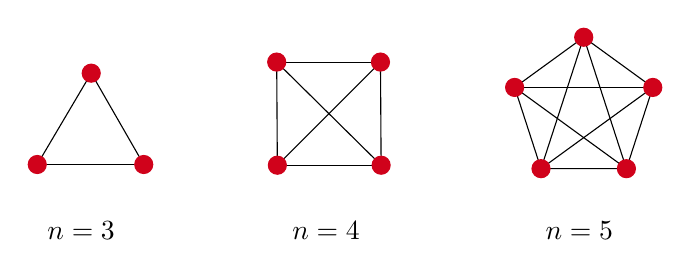
\begin{tikzpicture}[x=0.75pt,y=0.75pt,yscale=-1,xscale=1]
  %uncomment if require: \path (0,244); %set diagram left start at 0, and has height of 244
  
  %Straight Lines [id:da9981694225390096] 
  \draw    (259.71,56.31) -- (210.02,106) ;
  %Straight Lines [id:da26707606947695417] 
  \draw    (209.71,56.31) -- (260.02,106) ;
  %Straight Lines [id:da6585835091291369] 
  \draw    (209.71,56.31) -- (210.02,106) ;
  %Straight Lines [id:da7219351678460844] 
  \draw    (259.71,56.31) -- (260.02,106) ;
  %Straight Lines [id:da0019303873533728089] 
  \draw    (209.71,56.31) -- (259.71,56.31) ;
  %Straight Lines [id:da7049983363855998] 
  \draw    (210.02,106) -- (260.02,106) ;
  %Straight Lines [id:da35560926010509697] 
  \draw    (120.35,61.65) -- (94.35,105.65) ;
  %Straight Lines [id:da7897834071428548] 
  \draw    (120.35,61.65) -- (145.65,105.65) ;
  %Straight Lines [id:da9938696204324634] 
  \draw    (94.35,105.65) -- (145.65,105.65) ;
  %Shape: Ellipse [id:dp4113314666492133] 
  \draw  [color={rgb, 255:red, 208; green, 2; blue, 27 }  ,draw opacity=1 ][fill={rgb, 255:red, 208; green, 2; blue, 27 }  ,fill opacity=1 ] (90,105.65) .. controls (90,103.26) and (91.95,101.31) .. (94.35,101.31) .. controls (96.74,101.31) and (98.69,103.26) .. (98.69,105.65) .. controls (98.69,108.05) and (96.74,110) .. (94.35,110) .. controls (91.95,110) and (90,108.05) .. (90,105.65) -- cycle ;
  %Shape: Ellipse [id:dp834167188739953] 
  \draw  [color={rgb, 255:red, 208; green, 2; blue, 27 }  ,draw opacity=1 ][fill={rgb, 255:red, 208; green, 2; blue, 27 }  ,fill opacity=1 ] (141.31,105.65) .. controls (141.31,103.26) and (143.26,101.31) .. (145.65,101.31) .. controls (148.05,101.31) and (150,103.26) .. (150,105.65) .. controls (150,108.05) and (148.05,110) .. (145.65,110) .. controls (143.26,110) and (141.31,108.05) .. (141.31,105.65) -- cycle ;
  %Shape: Ellipse [id:dp8095001658436142] 
  \draw  [color={rgb, 255:red, 208; green, 2; blue, 27 }  ,draw opacity=1 ][fill={rgb, 255:red, 208; green, 2; blue, 27 }  ,fill opacity=1 ] (116,61.65) .. controls (116,59.26) and (117.95,57.31) .. (120.35,57.31) .. controls (122.74,57.31) and (124.69,59.26) .. (124.69,61.65) .. controls (124.69,64.05) and (122.74,66) .. (120.35,66) .. controls (117.95,66) and (116,64.05) .. (116,61.65) -- cycle ;
  %Shape: Ellipse [id:dp10911439146709467] 
  \draw  [color={rgb, 255:red, 208; green, 2; blue, 27 }  ,draw opacity=1 ][fill={rgb, 255:red, 208; green, 2; blue, 27 }  ,fill opacity=1 ] (205.37,56.31) .. controls (205.37,53.91) and (207.31,51.96) .. (209.71,51.96) .. controls (212.11,51.96) and (214.06,53.91) .. (214.06,56.31) .. controls (214.06,58.71) and (212.11,60.65) .. (209.71,60.65) .. controls (207.31,60.65) and (205.37,58.71) .. (205.37,56.31) -- cycle ;
  %Shape: Ellipse [id:dp8819360357436353] 
  \draw  [color={rgb, 255:red, 208; green, 2; blue, 27 }  ,draw opacity=1 ][fill={rgb, 255:red, 208; green, 2; blue, 27 }  ,fill opacity=1 ] (255.37,56.31) .. controls (255.37,53.91) and (257.31,51.96) .. (259.71,51.96) .. controls (262.11,51.96) and (264.06,53.91) .. (264.06,56.31) .. controls (264.06,58.71) and (262.11,60.65) .. (259.71,60.65) .. controls (257.31,60.65) and (255.37,58.71) .. (255.37,56.31) -- cycle ;
  %Shape: Ellipse [id:dp05860712986316774] 
  \draw  [color={rgb, 255:red, 208; green, 2; blue, 27 }  ,draw opacity=1 ][fill={rgb, 255:red, 208; green, 2; blue, 27 }  ,fill opacity=1 ] (205.68,106) .. controls (205.68,103.6) and (207.62,101.65) .. (210.02,101.65) .. controls (212.42,101.65) and (214.37,103.6) .. (214.37,106) .. controls (214.37,108.4) and (212.42,110.35) .. (210.02,110.35) .. controls (207.62,110.35) and (205.68,108.4) .. (205.68,106) -- cycle ;
  %Shape: Ellipse [id:dp5283352169897437] 
  \draw  [color={rgb, 255:red, 208; green, 2; blue, 27 }  ,draw opacity=1 ][fill={rgb, 255:red, 208; green, 2; blue, 27 }  ,fill opacity=1 ] (255.68,106) .. controls (255.68,103.6) and (257.62,101.65) .. (260.02,101.65) .. controls (262.42,101.65) and (264.37,103.6) .. (264.37,106) .. controls (264.37,108.4) and (262.42,110.35) .. (260.02,110.35) .. controls (257.62,110.35) and (255.68,108.4) .. (255.68,106) -- cycle ;
  %Shape: Regular Polygon [id:dp10308828814670479] 
  \draw   (357.63,44.35) -- (390.92,68.53) -- (378.2,107.66) -- (337.06,107.66) -- (324.35,68.53) -- cycle ;
  %Straight Lines [id:da43627704398128486] 
  \draw    (324.35,68.53) -- (378.2,107.66) ;
  %Straight Lines [id:da0011702067257907123] 
  \draw    (337.06,107.66) -- (390.92,68.53) ;
  %Straight Lines [id:da9427395129530866] 
  \draw    (337.06,107.66) -- (357.63,44.35) ;
  %Straight Lines [id:da7244564555034867] 
  \draw    (324.35,68.53) -- (390.92,68.53) ;
  %Straight Lines [id:da6627152022664105] 
  \draw    (357.63,44.35) -- (378.2,107.66) ;
  %Shape: Ellipse [id:dp7300400411305249] 
  \draw  [color={rgb, 255:red, 208; green, 2; blue, 27 }  ,draw opacity=1 ][fill={rgb, 255:red, 208; green, 2; blue, 27 }  ,fill opacity=1 ] (353.29,44.35) .. controls (353.29,41.95) and (355.23,40) .. (357.63,40) .. controls (360.03,40) and (361.98,41.95) .. (361.98,44.35) .. controls (361.98,46.74) and (360.03,48.69) .. (357.63,48.69) .. controls (355.23,48.69) and (353.29,46.74) .. (353.29,44.35) -- cycle ;
  %Shape: Ellipse [id:dp8020435268234443] 
  \draw  [color={rgb, 255:red, 208; green, 2; blue, 27 }  ,draw opacity=1 ][fill={rgb, 255:red, 208; green, 2; blue, 27 }  ,fill opacity=1 ] (320,68.53) .. controls (320,66.13) and (321.95,64.18) .. (324.35,64.18) .. controls (326.74,64.18) and (328.69,66.13) .. (328.69,68.53) .. controls (328.69,70.93) and (326.74,72.87) .. (324.35,72.87) .. controls (321.95,72.87) and (320,70.93) .. (320,68.53) -- cycle ;
  %Shape: Ellipse [id:dp5063058740897554] 
  \draw  [color={rgb, 255:red, 208; green, 2; blue, 27 }  ,draw opacity=1 ][fill={rgb, 255:red, 208; green, 2; blue, 27 }  ,fill opacity=1 ] (332.71,107.66) .. controls (332.71,105.26) and (334.66,103.32) .. (337.06,103.32) .. controls (339.46,103.32) and (341.4,105.26) .. (341.4,107.66) .. controls (341.4,110.06) and (339.46,112.01) .. (337.06,112.01) .. controls (334.66,112.01) and (332.71,110.06) .. (332.71,107.66) -- cycle ;
  %Shape: Ellipse [id:dp20023345004172588] 
  \draw  [color={rgb, 255:red, 208; green, 2; blue, 27 }  ,draw opacity=1 ][fill={rgb, 255:red, 208; green, 2; blue, 27 }  ,fill opacity=1 ] (373.86,107.66) .. controls (373.86,105.26) and (375.8,103.32) .. (378.2,103.32) .. controls (380.6,103.32) and (382.55,105.26) .. (382.55,107.66) .. controls (382.55,110.06) and (380.6,112.01) .. (378.2,112.01) .. controls (375.8,112.01) and (373.86,110.06) .. (373.86,107.66) -- cycle ;
  %Shape: Ellipse [id:dp34706748597281534] 
  \draw  [color={rgb, 255:red, 208; green, 2; blue, 27 }  ,draw opacity=1 ][fill={rgb, 255:red, 208; green, 2; blue, 27 }  ,fill opacity=1 ] (386.57,68.53) .. controls (386.57,66.13) and (388.52,64.18) .. (390.92,64.18) .. controls (393.32,64.18) and (395.26,66.13) .. (395.26,68.53) .. controls (395.26,70.93) and (393.32,72.87) .. (390.92,72.87) .. controls (388.52,72.87) and (386.57,70.93) .. (386.57,68.53) -- cycle ;
  
  % Text Node
  \draw (98,132) node [anchor=north west][inner sep=0.75pt]    {$n=3$};
  % Text Node
  \draw (216,132) node [anchor=north west][inner sep=0.75pt]    {$n=4$};
  % Text Node
  \draw (338,132) node [anchor=north west][inner sep=0.75pt]    {$n=5$};
  
  
  \end{tikzpicture}
  
    \end{center}
    Note that there is an edge between every pair of vertices.
  \end{definition}

\end{frame}

\begin{frame}
  \frametitle{A Remark on Conventions}

  \textbf{Remark}.
    In our definition of a graph, we {\itshape don't allow} loops, and there {\itshape cannot} be multiple edges between the same set of vertices.
    \begin{center}
      
  
  \tikzset{every picture/.style={line width=0.75pt}} %set default line width to 0.75pt        
  
  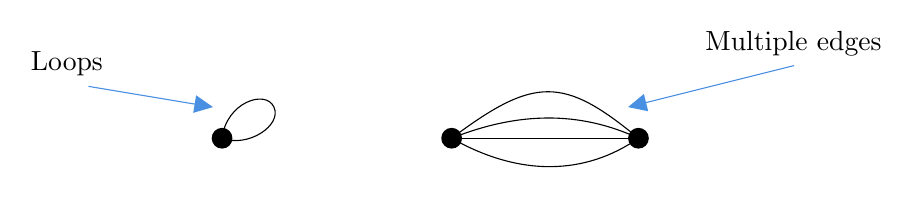
\begin{tikzpicture}[x=0.75pt,y=0.75pt,yscale=-1,xscale=1]
  %uncomment if require: \path (0,93); %set diagram left start at 0, and has height of 93
  
  %Curve Lines [id:da2865357772607766] 
  \draw    (194.39,55) .. controls (196.39,37.75) and (215.39,31.25) .. (219.39,40) .. controls (223.39,48.75) and (206.89,59.75) .. (194.39,55) -- cycle ;
  %Shape: Circle [id:dp0229132580239656] 
  \draw  [draw opacity=0][fill={rgb, 255:red, 0; green, 0; blue, 0 }  ,fill opacity=1 ] (189.39,55) .. controls (189.39,52.24) and (191.63,50) .. (194.39,50) .. controls (197.15,50) and (199.39,52.24) .. (199.39,55) .. controls (199.39,57.76) and (197.15,60) .. (194.39,60) .. controls (191.63,60) and (189.39,57.76) .. (189.39,55) -- cycle ;
  %Shape: Circle [id:dp1638222573350646] 
  \draw  [draw opacity=0][fill={rgb, 255:red, 0; green, 0; blue, 0 }  ,fill opacity=1 ] (300,55) .. controls (300,52.24) and (302.24,50) .. (305,50) .. controls (307.76,50) and (310,52.24) .. (310,55) .. controls (310,57.76) and (307.76,60) .. (305,60) .. controls (302.24,60) and (300,57.76) .. (300,55) -- cycle ;
  %Shape: Circle [id:dp537703730076633] 
  \draw  [draw opacity=0][fill={rgb, 255:red, 0; green, 0; blue, 0 }  ,fill opacity=1 ] (390,55) .. controls (390,52.24) and (392.24,50) .. (395,50) .. controls (397.76,50) and (400,52.24) .. (400,55) .. controls (400,57.76) and (397.76,60) .. (395,60) .. controls (392.24,60) and (390,57.76) .. (390,55) -- cycle ;
  %Straight Lines [id:da6617588206410779] 
  \draw    (305,55) -- (395,55) ;
  %Curve Lines [id:da23655718519286506] 
  \draw    (305,55) .. controls (345,25) and (359,25.25) .. (395,55) ;
  %Curve Lines [id:da6706610581979621] 
  \draw    (305,55) .. controls (337,42.25) and (366.5,41.75) .. (395,55) ;
  %Curve Lines [id:da14619136331292015] 
  \draw    (305,55) .. controls (338,73.75) and (369.5,72.75) .. (395,55) ;
  %Straight Lines [id:da03138886450780565] 
  \draw [color={rgb, 255:red, 74; green, 144; blue, 226 }  ,draw opacity=1 ]   (130,30) -- (187.04,39.51) ;
  \draw [shift={(190,40)}, rotate = 189.46] [fill={rgb, 255:red, 74; green, 144; blue, 226 }  ,fill opacity=1 ][line width=0.08]  [draw opacity=0] (8.93,-4.29) -- (0,0) -- (8.93,4.29) -- cycle    ;
  %Straight Lines [id:da17643117622964488] 
  \draw [color={rgb, 255:red, 74; green, 144; blue, 226 }  ,draw opacity=1 ]   (470,20) -- (392.91,39.27) ;
  \draw [shift={(390,40)}, rotate = 345.96000000000004] [fill={rgb, 255:red, 74; green, 144; blue, 226 }  ,fill opacity=1 ][line width=0.08]  [draw opacity=0] (8.93,-4.29) -- (0,0) -- (8.93,4.29) -- cycle    ;
  
  % Text Node
  \draw (101,12) node [anchor=north west][inner sep=0.75pt]   [align=left] {Loops};
  % Text Node
  \draw (426,2) node [anchor=north west][inner sep=0.75pt]   [align=left] {Multiple edges};
  
  
  \end{tikzpicture}
  
    \end{center}
    
    You can define graphs where such things are allowed, but for now we will outlaw them. We also note that edges are \emph{unordered pairs}, so for now edges have no direction.
  

\end{frame}

\begin{frame}
  \frametitle{Notation}

  \textbf{Notation}. If $G=(V, E)$ is a graph, and we have some edge $\{x, y\} \in E$, we will denote it by $x y$. We will also define $|G|=|V|$, and $e(G)=|E|$.

  \vspace*{1.25cm}

  \begin{example}
    How many vertices and edges does the graph $K_n$ have?

    % \vspace*{2\baselineskip}
    % \pause


    % We have $|K_n| = n$ and $e(K_n) = \binom{k}{2}$, as there is an edge between any pair of vertices.
    
  \end{example}

  \pause

  \emph{Solution}. We have $|K_n| = n$ and $e(K_n) = \binom{k}{2}$, as there is an edge between any pair of vertices.

\end{frame}


\end{document}